\chapter{Molecular dipole moments}
\label{ch:t-dipoles}
\index{Dipole moment}
\index{Bond dipole}
\index{Carbon dioxide}\index{Sulfur dioxide}\index{Water}
\eccexample{Examples > General Chemistry > Polar bonds and dipole moments}

Students learn that a molecule with polar bonds can still be non-polar, and that the shape decides. This chapter gives the teacher the numbers to show it: the charges on the atoms, which say how polar each bond is, next to the dipole moment of the whole molecule, which says whether the bond dipoles cancel. \chem{CO2} and \chem{SO2} make the central pair, two molecules with the same kind of bonds, one linear and one bent, and \chem{BF3}, \chem{CH4} and \chem{SF6} show the same cancellation in three dimensions.

\section*{This requires}
Nothing beyond ECCE: the calculations are in the General Chemistry example set.

\section{The calculations}
All eight molecules are in the topic \menu{Polar bonds and dipole moments}: \emph{CO2}, \emph{SO2}, \emph{CH3F}, \emph{H2O\_dipole}, \emph{NH3\_dipole}, \emph{BF3\_dipole}, \emph{CH4\_dipole} and \emph{SF6\_dipole}. Each is a single molecule in the gas phase at its optimised structure, and all were calculated in the same way, with a basis set chosen to give good dipole moments.

\section{Procedure}
\begin{enumerate}
	\item In the Organizer, choose \menu{File > Open Example Calculations}, pick \menu{General Chemistry} and click \menu{OK}.
	\item Open \emph{CO2} in the Viewer. Open \menu{Properties > Charges > CHELPG / ESP-Fitted Charges} to see the charge on each atom, and \menu{Properties > Electric properties > Dipole Moment} for the dipole moment of the molecule.
	\item With \menu{Measure} (Chapter~\ref{ch:first-calculation}), measure the angle O--C--O.
	\item Repeat for \emph{SO2} (angle O--S--O), \emph{H2O\_dipole} (H--O--H), \emph{NH3\_dipole}, \emph{CH3F}, \emph{BF3\_dipole}, \emph{CH4\_dipole} and \emph{SF6\_dipole}.
	\item In \emph{CO2}, \emph{SO2} and \emph{H2O\_dipole}, open \menu{Properties > Orbitals > MOs}, choose \menu{ESP on Density} in the box next to \menu{Compute} and click \menu{Compute}.
\end{enumerate}
\index{Dipole moment!showing}\index{Charges!ESP-fitted}

\section{Polar bonds, polar molecules}
The charges are the ones that best reproduce the electric field the calculated molecule produces around itself, so they say how the molecule looks to a neighbouring charge; a positive number means the atom has given up part of an electron. The dipole moment is in debye (D): one debye is about a fifth of the dipole of one electron and one proton \SI{1}{\angstrom} apart.

\begin{table}[htbp]
	\centering
	\caption{Charge on the central atom (in units of the proton charge), bond angle and dipole moment $\mu$ of eight molecules. Calculated values from the stored ECCE calculations; measured dipole moments in the gas phase from the NIST CCCBDB \cite{cccbdb}. A dash means the molecule's symmetry makes the dipole moment exactly zero.}
	\label{tab:dp}
	\begin{tabular}{lrrrr}
		\toprule
		Molecule & central atom charge & angle & $\mu$ calc.\ (D) & $\mu$ meas.\ (D) \\
		\midrule
		\chem{CO2} & C $+0.78$ & \ang{180} & 0 & -- \\
		\chem{BF3} & B $+0.91$ & \ang{120} & 0 & -- \\
		\chem{CH4} & C $-0.32$ & \ang{109.5} & 0 & -- \\
		\chem{SF6} & S $+0.59$ & \ang{90} & 0 & -- \\
		\chem{SO2} & S $+0.59$ & \ang{117.5} & 1.92 & 1.63 \\
		\chem{H2O} & O $-0.67$ & \ang{104.7} & 1.85 & 1.86 \\
		\chem{NH3} & N $-0.85$ & \ang{106.8} & 1.52 & 1.48 \\
		\chem{CH3F} & F $-0.26$ & & 1.91 & 1.85 \\
		\bottomrule
	\end{tabular}
\end{table}

Table~\ref{tab:dp} shows that the first four molecules have strongly charged central atoms and still no dipole moment, because their bonds point symmetrically in opposite directions and the bond dipoles cancel. In \chem{CO2} the carbon carries $+0.78$ and each oxygen $-0.39$, so each C=O bond is clearly polar, but the two bonds point away from carbon along one line, and the two bond dipoles, equal in size and opposite in direction, add up to zero. In \chem{BF3} three bond dipoles at \ang{120} cancel in the plane, and in \chem{CH4} and \chem{SF6} four and six cancel in space. Hence a molecule is non-polar whenever its polar bonds are arranged so that the centre of the negative charge falls on the centre of the positive charge.

\chem{SO2} has the same kind of bonds as \chem{CO2}, sulfur positive and oxygen negative, but it is bent at \ang{117.5}, and its dipole moment is 1.92~D (measured 1.63~D). The two bond dipoles now point partly the same way, toward the side of the oxygen atoms, and no longer cancel. Hence the shape, and not the bonds alone, decides whether a molecule is polar; why \chem{SO2} is bent and \chem{CO2} is not is the subject of Chapter~\ref{ch:t-shapes}.

\section{Where the dipole moment comes from}
The dipole moment that ECCE shows is worked out from the whole charge of the molecule: each nucleus is a positive point charge at its position, and the electrons are a cloud of negative charge spread over the molecule, the electron density of the calculation. Each piece of charge is multiplied by its position and all of them are added up. For a neutral molecule the result does not depend on where the positions are measured from, and it is zero exactly when the centre of the positive charge and the centre of the negative charge fall on the same point. In physics the dipole points from the centre of negative charge to the centre of positive charge; chemists usually draw the arrow the other way, towards the negative end, as in the figures of this chapter.
\index{Dipole moment!how it is calculated}

Bond dipoles are a way of splitting this one vector into pieces a class can draw. Give each atom its charge from the table and take the outer atom of each bond: its charge times the bond, as an arrow along the bond, is that bond's dipole. Added as arrows, head to tail, the bond dipoles of a neutral molecule give exactly the dipole of the atomic charges, and that is close to the dipole moment worked out from the whole charge cloud: for water 1.90~D against 1.85~D.

\begin{figure}[htbp]
	\centering
	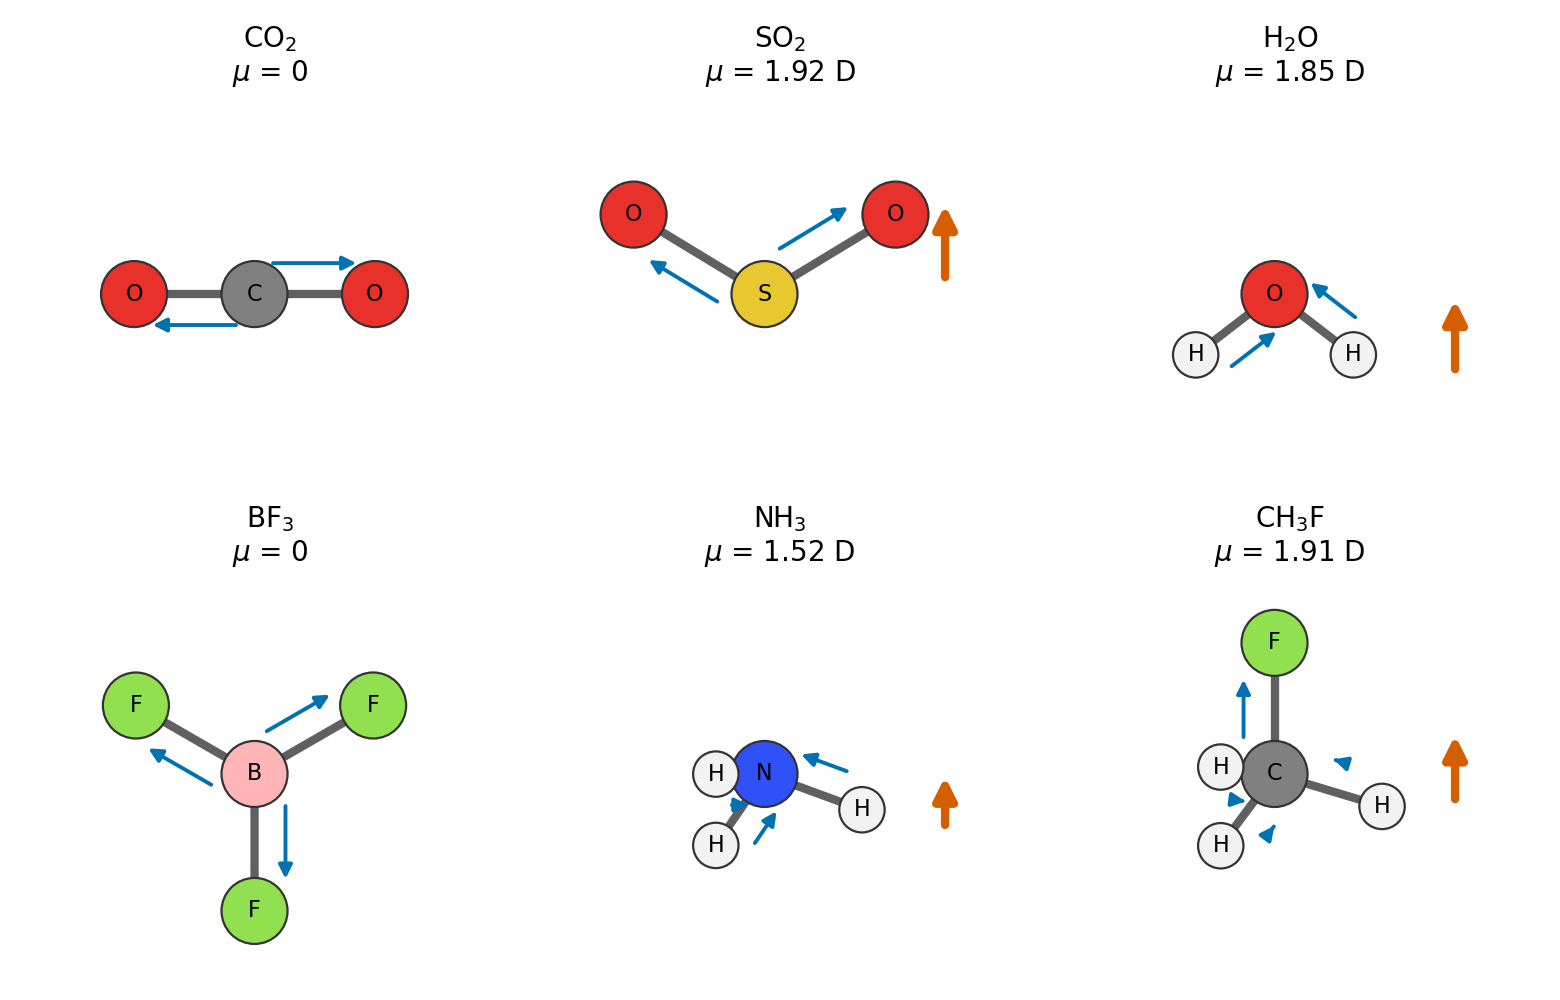
\includegraphics[width=0.95\linewidth]{dipoles/bond-dipoles.ecce-9.5.3-dev.png}
	\caption{Bond dipoles (thin blue arrows, one beside each bond) and the dipole moment of the whole molecule (thick orange arrow, drawn beside the molecule) of six of the molecules of table~\ref{tab:dp}, all pointing towards the negative end. Each bond dipole is the charge of its outer atom times the bond, from the stored atomic charges; the molecular dipole is the calculated dipole moment, at the same scale. \chem{NH3} and \chem{CH3F} are seen from a little above, so that all their atoms show. Drawn from the stored ECCE results.}
	\label{fig:dp-arrows}
\end{figure}

Figure~\ref{fig:dp-arrows} shows the bond dipoles of \chem{CO2} pointing away from each other along one line and those of \chem{BF3} pointing to the corners of a triangle, while those of \chem{SO2}, \chem{H2O}, \chem{NH3} and \chem{CH3F} all lean towards one side of the molecule. This is because the arrows add head to tail: two equal arrows in opposite directions, or three at \ang{120}, end where they started, while arrows that share a direction leave a sum. Hence the thick arrow appears only on the bent and pyramidal molecules and on \chem{CH3F}, whose one strong C--F bond dipole is not balanced by the three weak C--H ones.

\begin{figure}[htbp]
	\centering
	\begin{tabular}{ccc}
		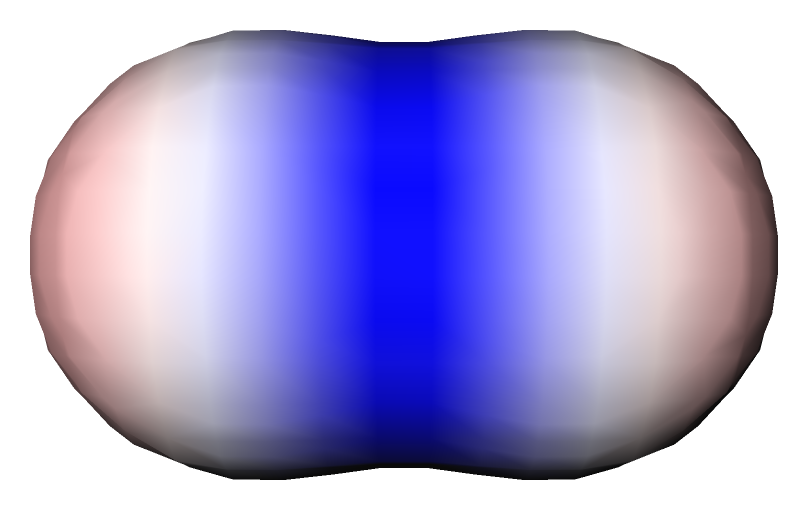
\includegraphics[height=2.6cm]{dipoles/co2-esp.ecce-9.5.3-dev.png} &
		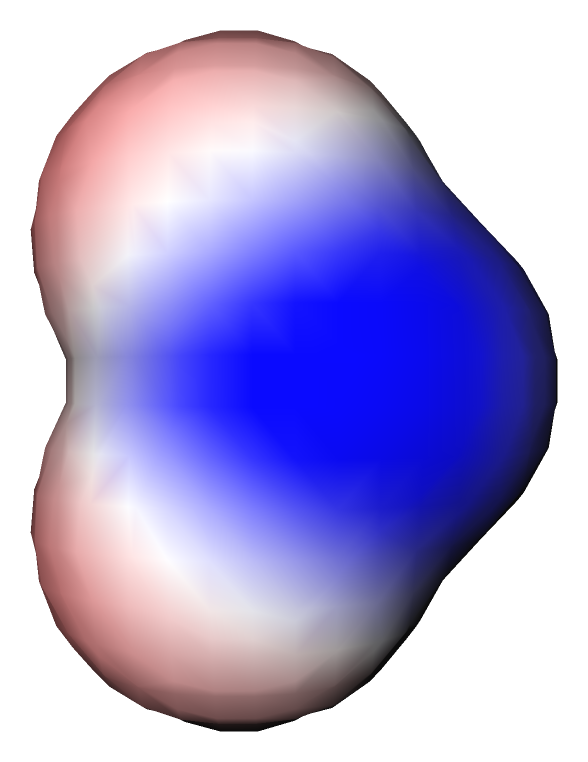
\includegraphics[height=2.6cm]{dipoles/so2-esp.ecce-9.5.3-dev.png} &
		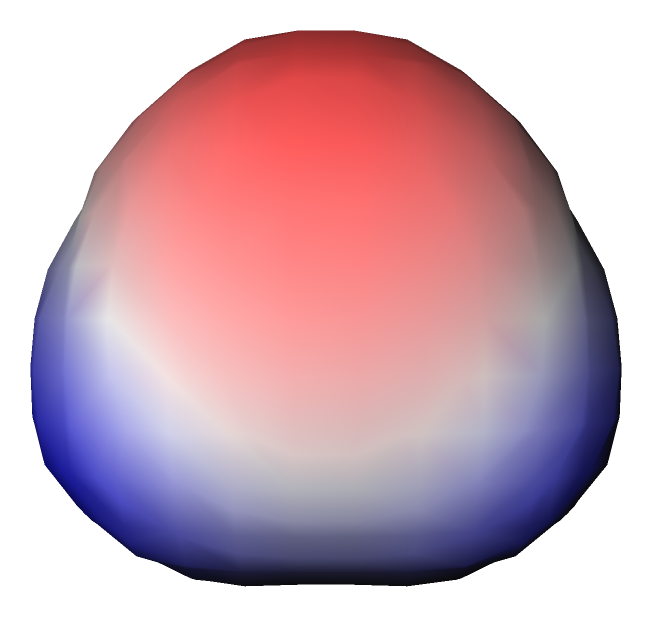
\includegraphics[height=2.6cm]{dipoles/h2o-esp.ecce-9.5.3-dev.png} \\
		\chem{CO2} & \chem{SO2} & \chem{H2O} \\
	\end{tabular}
	\caption{The electric potential on a surface of constant electron density (\menu{ESP on Density} in the \menu{MOs} panel), red negative and blue positive, each picture on its own colour scale (\menu{ESP range: Auto}). \chem{CO2}: the O atoms at the left and right ends, C in the middle. \chem{SO2}: the two O atoms on the left, S on the right. \chem{H2O}: O at the top, the two H atoms at the lower corners.}
	\label{fig:dp-esp}
\end{figure}

Figure~\ref{fig:dp-esp} shows where the charge sits on the outside of each molecule. \chem{CO2} is red at both ends and blue round the middle, symmetric front to back, while \chem{SO2} and \chem{H2O} are red on one side and blue on the other, because a straight molecule puts its negative oxygen atoms at the two ends and a bent one puts them on the same side. Hence a molecule with one red side and one blue side has a dipole moment, and a molecule whose colours are arranged symmetrically has none, which a class can judge from the picture before reading the number.

\section{Adding bond dipoles}
For a bent molecule with two equal bonds the addition can be done on the board. Each bond dipole $\mu_\mathrm{b}$ points along its bond; the components across the molecule cancel and the components along the axis add, so $\mu = 2\mu_\mathrm{b}\cos(\theta/2)$, where $\theta$ is the bond angle. With the calculated values, water ($\mu = 1.85$~D, $\theta = \ang{104.7}$) has a bond dipole of 1.52~D per O--H bond, and \chem{SO2} ($\mu = 1.92$~D, $\theta = \ang{117.5}$) one of 1.85~D per S=O bond. This shows that the bond dipoles of the two molecules are of a similar size, because both bonds join an electronegative atom to a less electronegative one. Hence the angle decides most of the difference between bent and straight molecules: the factor $\cos(\theta/2)$ is 0.61 at \ang{104.7}, 0.52 at \ang{117.5}, and at \ang{180}, the angle of \chem{CO2}, it is zero.
\index{Bond dipole!addition}

The calculated dipole moments of \chem{H2O}, \chem{NH3} and \chem{CH3F} are within 3\,\% of the measured ones; that of \chem{SO2} is 18\,\% too large, so in the calculated column \chem{SO2} comes out as the most polar of the four, while measured it is third. The zeros of the symmetric molecules and the contrast between \chem{CO2} and \chem{SO2} hold exactly in both columns; to rank the four polar molecules, use the measured one.

\section{In class}
Show \chem{CO2} and \chem{SO2} side by side with their charges switched on or their ESP surfaces drawn, ask whether each molecule is polar, and then show the dipole moments. Draw the two bond dipoles as arrows on each molecule; the class can see that the arrows of \chem{CO2} point away from each other along one line and those of \chem{SO2} add up.

\section{History}
Debye introduced the permanent dipole moment of a molecule in 1912 to explain how the dielectric constant of a substance depends on temperature \cite{debye1912}, and collected the theory and the measured values in his book \emph{Polar Molecules} of 1929 \cite{debye1929}.
\index{Debye, Peter}
